\documentclass[a4paper,BCOR=5mm,oneside,openany]{scrreprt}
\usepackage{fontspec}
\usepackage{lmodern}
\usepackage{amsmath,amsthm,mathtools}
\usepackage{amsfonts,amssymb}
\usepackage{graphicx,overpic}
\usepackage{hyperref}
\usepackage{microtype}
\usepackage{dsfont}
\usepackage{booktabs}
\usepackage{fullpage}
\usepackage{float}
\usepackage{subfig}
%\usepackage{minted}
\usepackage[style=philosophy-modern,
            hyperref,backref,natbib,
            backend=biber]{biblatex}
\bibliography{Biblio}
\usepackage{scrlayer-scrpage}
\pagestyle{scrheadings}
\usepackage{algorithm}
\usepackage{algpseudocode}
\usepackage[disable]{todonotes}
\usepackage{subfloat}
%% Header
\setheadsepline{.4pt}
\clearscrheadings
\automark[chapter]{chapter}
\ihead{\headmark}
\ohead[\pagemark]{\pagemark}
\cfoot[]{}
%% Footer
\usepackage[bottom=2cm,footskip=8mm,head=13.6pt]{geometry}
\usepackage{pgfplots}

\pgfplotsset{compat=1.14}
\pgfplotsset{grid style={solid,black}}
\pgfplotsset{minor grid style={dashed,black}}
%% Font
%\usepackage[fullfamily,opticals,onlymath]{MinionPro}
%\setmainfont{Minion Pro}


\DeclareCiteCommand{\footpartcite}[\mkbibfootnote]
  {\usebibmacro{prenote}}
  {\usebibmacro{citeindex}%
   %\mkbibbrackets{\usebibmacro{cite}}%
   %\setunit{\addnbspace}
   \printnames{labelname}%
   \setunit{\labelnamepunct}
   \printfield[citetitle]{title}%
   \newunit
   \printfield{year}}
  {\addsemicolon\space}
  {\usebibmacro{postnote}}
  
\hypersetup{
    colorlinks,
    linkcolor={red!50!black},
    citecolor={blue!50!black},
    urlcolor={blue!80!black},
    linktoc=page
}

\graphicspath{{images/}}

\newcommand{\sgn}{\operatorname{sgn}}
\newcommand{\conv}{\operatorname{conv}}
\newcommand{\vect}{\operatorname{vect}}
\DeclareMathOperator*{\argmin}{arg\,min}
\DeclareMathOperator*{\argmax}{arg\,max}
\newcommand*\diff{\mathop{}\!\mathrm{d}}
\newcommand{\Var}{\mathrm{Var}}
\newcommand*\ri{\mathop{}\!\mathrm{ri}}
\newcommand*\aff{\mathop{}\!\mathrm{aff}}
\newcommand*\dom{\mathop{}\!\mathrm{dom}}
\newcommand*\epi{\mathop{}\!\mathrm{epi}}
\newcommand*\diag{\mathop{}\!\mathrm{diag}}
\newcommand*\cov{\mathop{}\!\mathrm{cov}}
\newcommand*\var{\mathop{}\!\mathrm{var}}
\newcommand*\corr{\mathop{}\!\mathrm{corr}}
\newcommand*\tr{\mathop{}\!\mathrm{tr}}


\begin{document}
%%%%%%%%%%%%%%%%%%%%%%%%%%%%%%%%%%%%%%%%%
% University Assignment Title Page 
% LaTeX Template
% Version 1.0 (27/12/12)
%
% This template has been downloaded from:
% http://www.LaTeXTemplates.com
%
% Original author:
% WikiBooks (http://en.wikibooks.org/wiki/LaTeX/Title_Creation)
%
% License:
% CC BY-NC-SA 3.0 (http://creativecommons.org/licenses/by-nc-sa/3.0/)
% 
% Instructions for using this template:
% This title page is capable of being compiled as is. This is not useful for 
% including it in another document. To do this, you have two options: 
%
% 1) Copy/paste everything between \begin{document} and \end{document} 
% starting at \begin{titlepage} and paste this into another LaTeX file where you 
% want your title page.
% OR
% 2) Remove everything outside the \begin{titlepage} and \end{titlepage} and 
% move this file to the same directory as the LaTeX file you wish to add it to. 
% Then add \input{./title_page_1.tex} to your LaTeX file where you want your
% title page.
%
%%%%%%%%%%%%%%%%%%%%%%%%%%%%%%%%%%%%%%%%%

%----------------------------------------------------------------------------------------
%	PACKAGES AND OTHER DOCUMENT CONFIGURATIONS
%----------------------------------------------------------------------------------------
\begin{titlepage}

\newcommand{\HRule}{\rule{\linewidth}{0.5mm}} % Defines a new command for the horizontal lines, change thickness here

\center % Center everything on the page
 
%----------------------------------------------------------------------------------------
%	HEADING SECTIONS
%----------------------------------------------------------------------------------------

%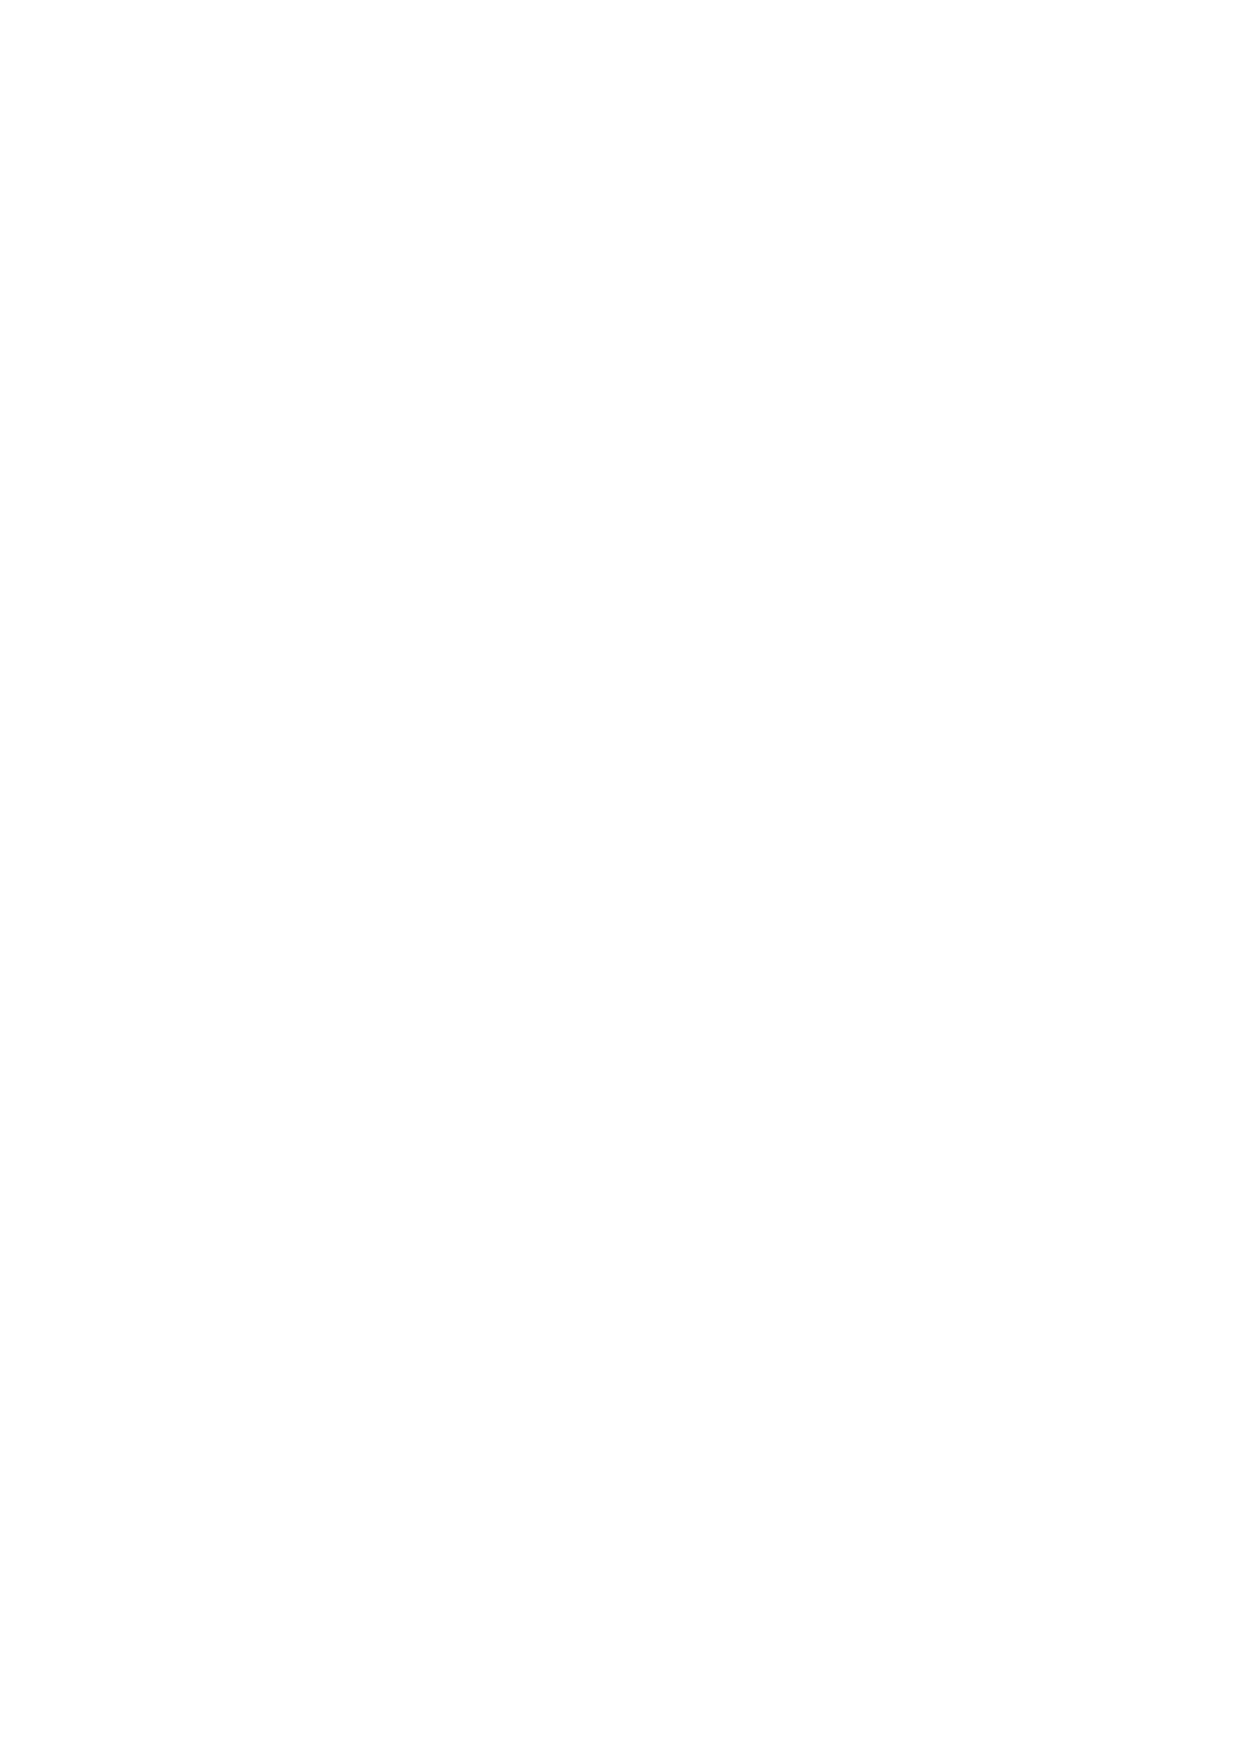
\includegraphics[width=0.15\textwidth]{logo.svg}~\\[1cm] % Logo

\textsc{\LARGE Université Paris Dauphine}\\[1.5cm] % Name of your university/college
\textsc{\Large Probabilistic Graphical Models}\\[0.5cm] % Major heading such as course name

%----------------------------------------------------------------------------------------
%	TITLE SECTION
%----------------------------------------------------------------------------------------

\HRule \\[0.4cm]
{ \huge \bfseries Independent Component Analysis.
}\\[0.4cm] % Title of your document
\HRule \\[1.5cm]
 
%----------------------------------------------------------------------------------------
%	AUTHOR SECTION
%----------------------------------------------------------------------------------------

\begin{minipage}{0.4\textwidth}
\begin{flushleft} \large
\emph{Student:}\\
Guillaume \textsc{Ausset}
\end{flushleft}
\end{minipage}
~
\begin{minipage}{0.4\textwidth}
\begin{flushright} \large
\emph{Advisors:} \\
Francis \textsc{Bach} \\
Guillaume \textsc{Obozinski} % Supervisor's Name
\end{flushright}
\end{minipage}\\[4cm]

% If you don't want a supervisor, uncomment the two lines below and remove the section above
%\Large \emph{Author:}\\
%John \textsc{Smith}\\[3cm] % Your name

%----------------------------------------------------------------------------------------
%	DATE SECTION
%----------------------------------------------------------------------------------------

%{\large \today}\\[3cm] % Date, change the \today to a set date if you want to be precise

%----------------------------------------------------------------------------------------
%	LOGO SECTION
%----------------------------------------------------------------------------------------

%\includegraphics{Logo}\\[1cm] % Include a department/university logo - this will require the graphicx package
 
%----------------------------------------------------------------------------------------

\vfill % Fill the rest of the page with whitespace

\end{titlepage}

\tableofcontents

\chapter{The ICA framework}

\emph{All code, examples, images and any other material can be found in the \texttt{.zip} file provided. This zip file is actually a \texttt{Git} repository that can be found here: \url{https://github.com/aussetg/pgm-ica}. A notebook is available at \url{https://github.com/aussetg/pgm-ica/blob/master/examples/Experiments.ipynb}.}

\vspace{1cm}

In the physical world it is rare for the quantity of interest and the quantity measured to perfectly match. Scientists are used to dealing with measurements mixed with random noise but this is only one way information may be unavailable.
A very common situation is when our signal of interest, that we will from now on call $s \in \mathcal{R}^{m \times n}$ is actually mixed with itself. To try to recover our signal $s$ we will set up a certain number of recording devices, generally $n$ and from our recorded signals try to recover the sources. If we assume the sources are linearly mixed our problem is then:

\begin{align*}
	x = A s
\end{align*}

where $x \in \mathcal{R}^{k \times n}$, $A \in \mathcal{R}^{k \times m}$. While it is not necessarily the case or even needed from now on, we will assume $k = m$ so that the number of recorded signals equals the number of sources, the problem is then well posed.

If we somehow knew $A$ the mixing matrix then this problem would be easy to solve and one would only need to solve $s = A^{-1} x$, but in general it's impossible to obtain the matrix $A$ and the problem seems intractable, the number of unknowns dwarfing the number of known quantities.

We will see that in fact and quite surprisingly the sole hypothesis of the independence of the components of $s$ is enough to find a solution to the problem. 

There are, however, some limitations: because of the way the problem is posed one cannot hope to recover the real $s$ as for example a scaling or permutation of $A$ leaves the problem unchanged and we therefore cannot hope to recover the magnitudes (and therefore signs) of the $s_i$ or their order. We will also not be able to recover signals if more than $1$ is Gaussian as the distribution of the orthogonal transformation of a gaussian vector is the same as the original gaussian vector. See \cite{Hyvarinen2001} for a broader view of ICA.

\chapter{Preprocessing}

Before proceeding with the rest, we will quickly give two important preprocessing steps. 

This preprocessing has two important functions: it greatly simplifies the theory at no additional cost, and it while reduce the computational complexity.

\section{Centering}

The first step is to centre the $x$ such that $\mathbb{E} \left[ x \right] = 0$, we therefore just have to form $\tilde{x} = x -\mathbb{E} \left[ x \right]$.

This preprocessing greatly simplify the formulas and theory and have the advantage of not adding any constraint: once $W$ is found we only have to add back $W \mathbb{E} \left[ x \right]$ to the $s$ found.

We will also work with RKHS, we therefore reminds that is possible to find the gram matrix of the observations centered in the feature space without explicitly knowing how to centre in the feature space. In the rest of the report all kernel matrices will be considered centred that way. If we note $K$ the uncentred gram matrix then $\tilde{K}$ the centred gram matrix is given by:

\begin{align*}
	&H = \mathbb{I} - \frac{1}{N} \mathds{1_N} \\
  	&\tilde{K} = H K H
\end{align*}

\section{Whitening}\label{whitening}

ICA can be seen a generalization of PCA: while PCA gives uncorrelated components, ICA gives independent components. One implication of this fact is that an ICA solution is necessarily a PCA solution. It is therefore a good idea to first \emph{whiten} the data, i.e. diagonalize its covariance matrix before treating it with ICA.

The whitening process can be performed efficiently using the semi-definite positiveness of the covariance matrix by forming its eigenvalue decomposition:

\begin{align*}
	\mathbb{E} \left[ x x^\intercal \right] = U D U^\intercal
\end{align*}

Therefore if we note $P = U D^{-\frac{1}{2}} U^\intercal$, where $D^{-\frac{1}{2}}$ can be very efficiently computed, we have with $\tilde{x} = P x$

\begin{align*}
	\mathbb{E} \left[ x x^\intercal \right] = \mathbb{I}
\end{align*}

Computationally, this transformation has the advantage of making $W$ orthogonal, the parameters to estimate are therefore reduced from $n^2$ to $\frac{n (n-1)}{2}$. The new constraint "$W W^\intercal = \mathbb{I}$" also forces $W$ to lie on the Stiefel Manifold, giving very efficient optimization techniques.

\chapter{Measuring independence}

It is possible to treat the problem as a parametric one and to fix a certain form for the distributions but that case is quite limiting. We while therefore work in a semi-parametric framework with parameter $W$ the unmixing matrix:

\begin{align*}
	s = W y
\end{align*}

In the case $m = k$ we then have $W = A^{-1}$. It is natural to study $W$ directly as it is our parameter of interest and we will see that the problem is more easily expressed in terms of $W$.

We will suppose here that $m = k$ and $A$ is invertible to make this paragraph easier.

Given our semi-parametric formulation we want to find the maximum likelihood estimate of $A$. We will note $p^\star (x)$ the unknown ground truth of $x$ and $p(x)$ the model. Our problem is then:

\begin{align*}
	\text{minimize } D \left(p^\star(x) \mid \mid p(x) \right)
\end{align*}

We know that the KL divergence is invariant under an invertible transformation therefore the problem is equivalent to:

\begin{align*}
	\text{minimize } D \left(p^\star(s) \mid \mid p(s) \right)
\end{align*}

if we use the relation $x = A s$.

We also have the following relation:

\begin{align*}
	D(p^\star(s) \mid \mid p(s)) = D(p^\star(s) \mid \mid \tilde{p}(s)) + D( \tilde{p}(s) \mid \mid p(s))
\end{align*}

with $\tilde{p}(s)$ the product of the marginal densities of $p^\star(s)$ i.e. the density if the components were independent.

The minimum is then obtained for $p^\star(s) = \tilde{p}(s)$ and the problem is:

\begin{align*}
	\text{minimize } D \left(p^\star(x) \mid \mid \tilde{p}(s) \right)
\end{align*}

We want to minimize the \emph{mutual information between the components of $s$}.

A natural objective to optimize would therefore be the empirical mutual information of $s = W x$ but the empirical mutual information is complicated to compute, to make the problem tractable two different approaches are possible:

\begin{enumerate}
	\item Optimize an approximation of the mutual information.
	\item Optimize a \emph{contrast function} $J$, i.e a function with the same properties as the mutual information: $J(s) \geq 0, \forall s$ and $J(s) = 0$ iff the components of $s$ are independent.
\end{enumerate}

Fast-ICA will use the first approach while Kernel-ICA will use the second approach.

\chapter{A quick reminder of Fast-ICA}

We will use Fast-ICA as our reference algorithms as well as the method we will use to initialize our Kernel-ICA procedure. We therefore give a quick overview of the Fast-ICA algorithm.

Fast-ICA maximizes an approximation of the negentropy $J(s) = H(s_\text{gauss}) - H(s)$ which is equivalent to the minimizing the mutual information up to a constant.

Of course forming the empirical negentropy is equivalent to forming the empirical mutual information and the problem is therefore intractable. The approach taken is therefore to approximate the negentropy using non-linear functions.

In the case of non-quadratic function $G$, \cite{Hyvarinen1998}, proves that 

\begin{align*}
	J(s) \propto \left( \mathbb{E} \left[G(s) \right] - \mathbb{E} \left[ G(\nu) \right] \right)^2
\end{align*}

where $\nu \sim \mathcal{N}(0,1)$.

Two good (optimal in some sense) choices for $G$ are:

\begin{align*}
	&G_1 (u) = \log \cosh (a u) \\
	&G_2 (u) = −e^{-\frac{u^2}{2}}
\end{align*}

Fast-ICA is then a relatively simple fixed point algorithm obtained from the newton steps.

\begin{algorithm}
\caption{Fast-ICA} \label{fastica}
\begin{algorithmic}
    \Procedure{FastICA}{$X, G, \epsilon$}
    
    \State{$w \gets \textrm{Random orthogonal matrix}$}
    
    \While{ $1 - \min(\lvert \diag(w_i w_{i-1}^\intercal) \rvert) > \epsilon$ }
        \State{$w_{i+1} \gets G(w_{i} X) X^\intercal - \left(G'(w_{i} X) \mathds{1} \times \mathbb{I} \right) w_{i}$}
        \State{$w_{i+1} \gets (w_{i+1} w_{i+1}^\intercal)^{-\frac{1}{2}} w_{i+1}$}
    \EndWhile
    \State \Return $w, w X$
    \EndProcedure
\end{algorithmic}    
\end{algorithm}

By only working with matrix operations all computations can be done in-place and using a \texttt{BLAS}, making Fast-ICA extremely efficient.

\chapter{Kernel-ICA}

\section{Kernel contrast function}

We want to optimize a measure of independence of our estimated sources. Most approaches try to optimize an approximation of the mutual information. The measure chosen here by \cite{Bach2002} is for two variables:

\begin{align*}
	\rho_\mathcal{F} = \max_{f_1, f_2 \in \mathcal{F}} \corr (f_1(x_1), f_2 (x_2))
\end{align*}

We see that it is indeed a contrast function: it is always greater than $0$ and equal to $0$ iff the variables are independent if the family $\mathcal{F}$ is \emph{large enough} (if it includes Gaussian densities for example).

By exploiting the kernel trick we can obtain

\begin{align*}
	\rho_\mathcal{F} = \max_{f_1, f_2 \in \mathcal{F}} \corr ( \langle \Phi_1 (x_1), f_1 \rangle , \langle \Phi_2 (x_2), f_2 \rangle)
\end{align*}

We recognize a CCA problem and if we note $K_1$ and $K_2$ respective Gram matrices (assuming they are centred) we get the problem:

\begin{align*}
	\begin{pmatrix}
		0 & K_1 K_2 \\
		K_2 K_1 & 0
	\end{pmatrix} \begin{pmatrix}
		\alpha_1 \\ \alpha_2
	\end{pmatrix}
	= \rho \begin{pmatrix}
		K_1^2 & 0 \\
		0 & K_2^2
	\end{pmatrix} \begin{pmatrix}
		\alpha_1 \\ \alpha_2
	\end{pmatrix}
\end{align*}

This problem is unfortunately not well posed and will always be equal to $1$ for most kernels, we therefore adopt a regularized version as an estimator:

\begin{align*}
	\rho_\mathcal{F} = \max_{f_1, f_2 \in \mathcal{F}} \frac{\cov (f_1(x_1), f_2 (x_2))}{(\var f_1 (x_1) + \kappa \lVert f_1 \rVert^2 _\mathcal{F} )^{1/2} (\var f_2 (x_2) + \kappa \lVert f_2 \rVert^2 _\mathcal{F} )^{1/2}}
\end{align*}

The problem estimated at the first order is then:

\begin{align*}
	\begin{pmatrix}
		0 & K_1 K_2 \\
		K_2 K_1 & 0
	\end{pmatrix} \begin{pmatrix}
		\alpha_1 \\ \alpha_2
	\end{pmatrix}
	= \rho \begin{pmatrix}
		(K_1+\frac{N \kappa}{2} \mathbb{I})^2 & 0 \\
		0 & (K_2+\frac{N \kappa}{2} \mathbb{I})^2
	\end{pmatrix} \begin{pmatrix}
		\alpha_1 \\ \alpha_2
	\end{pmatrix}
\end{align*}

Of course we are interested in solving the $m$-variables problems, we can easily extend CCA to $m$ variables.

\begin{align*}
	&\begin{pmatrix}
		0 & K_1 K_2  & \cdots & K_1 K_m\\
		K_2 K_1 & 0 & \cdots & K_2 K_m \\
		\vdots & \vdots & \ddots & \vdots \\
		K_m K_1 & K_m K_2 & \cdots & 0
	\end{pmatrix} \begin{pmatrix}
		\alpha_1 \\ \alpha_2 \\ \vdots \\ \alpha_m
	\end{pmatrix} = \rho \begin{pmatrix}
		(K_1+\frac{N \kappa}{2} \mathbb{I})^2 & 0  & \cdots & 0\\
		0 & (K_2+\frac{N \kappa}{2} \mathbb{I})^2 & \cdots & 0 \\
		\vdots & \vdots & \ddots & \vdots \\
		0 & 0 & \cdots & (K_m+\frac{N \kappa}{2} \mathbb{I})^2
	\end{pmatrix} \begin{pmatrix}
		\alpha_1 \\ \alpha_2 \\ \vdots \\ \alpha_m
	\end{pmatrix}
\end{align*}

We can then transform that problem in the problem of finding the eigenvalues of:
						
\begin{align*}
	&\tilde{\mathcal{K}}_\kappa = \begin{pmatrix}
		\mathbb{I} & r_\kappa (K_1)  r_\kappa (K_2)  & \cdots &  r_\kappa (K_1) r_\kappa (K_m)\\
		r_\kappa (K_2)  r_\kappa (K_1) & \mathbb{I} & \cdots & r_\kappa (K_2) r_\kappa (K_m) \\
		\vdots & \vdots & \ddots & \vdots \\
		r_\kappa (K_m)  r_\kappa (K_1) & r_\kappa (K_m) r_\kappa (K_2) & \cdots & \mathbb{I}
	\end{pmatrix} \\
	& r_\kappa (K_i) = K_i (K_i + \frac{N \kappa}{2} \mathbb{I})^{-1}
\end{align*}

We then optimize:

\begin{align*}
	J(W) = -\frac{1}{2} \log C \left( \tilde{\mathcal{K}}_\kappa \right)
\end{align*}

With $C(U) = \det U$ for the KGV contrast function or $C(U) = \lambda_\text{min} (U)$ for KCCA. Both have strong links with the mutual information.

\section{Reducing complexity}

In practice the previous computation is intractable because of the dimensions involved and even forming the Gram matrices is impossible. We will therefore use the fact that the Gram matrices are semi-definite positive and use an incomplete Choleski decomposition to find a low rank approximation of the matrices involved.

\begin{algorithm}
\caption{Incomplete Choleski} \label{chol}
\begin{algorithmic}
    \Procedure{IncompleteCholeski}{$K \in \mathbb{R}^{n \times n}, \eta$}
    
    \State{$i, K', P \gets 1, K, \mathbb{I}$}
    \State{$G_{jj} \gets K_{jj}, \forall j$}
    
    \While{ $\sum_{j = 1}^n G_{jj} > \eta$ }
		\State{$j \gets \argmax_{j \in [1,n]} G_{jj}$}
		\State{$P_{ii} \gets 0 , P_{j^\star j^\star} \gets 0 , P_{ij^\star} \gets 1 , P_{j^\star i} \gets 1$}
		\State{$K_{1:n,i} \leftrightarrow K_{1:n,j^\star}$}
		\State{$K_{i,1:n} \leftrightarrow K_{j^\star, 1:n}$}
		\State{$G_{i,1:i} \leftrightarrow G_{j^\star, 1:i}$}
		\State{$G_{ii} = \sqrt{G_{jj}}$}
		\State{$G_{i+1:n,i} \gets \frac{1}{G_{ii}} \left( K'_{i+1:n, i} - \sum_{j=1}^{i-1} G_{i+1:n, j} G_{i,j} \right)$}
		\For{$j \in [i+1,n]$}
			\State{$G_{jj} = K_{jj} - \sum_{k = 1}^i G_{jk}^2$}
		\EndFor
		\State{$i \gets i + 1$}
    \EndWhile
    \State \Return $P, G, M = i-1$
    \EndProcedure
\end{algorithmic}    
\end{algorithm}

If we decompose the $K_i$ as
\begin{align*}
	K_i = G_i G_i^\intercal = U_i \Lambda_i U_i^\intercal
\end{align*}

with $\Lambda_i$ diagonal then if $R_i$ is $\Lambda_i$ regularized by $\lambda \to \frac{\lambda}{\lambda + N \kappa / 2}$ we have

\begin{align*}
	\tilde{\mathcal{K}}_\kappa = (\mathcal{U} \mathcal{V}) \begin{pmatrix}
		\mathcal{R}_\kappa & 0 \\
		0 & \mathbb{I}
	\end{pmatrix} (\mathcal{U} \mathcal{V})^\intercal
\end{align*}

with

\begin{align*}
	\mathcal{R}_\kappa =  \begin{pmatrix}
		\mathbb{I} & R_1 U_1^\intercal U_2 R_2  & \cdots &  R_1 U_1^\intercal U_m R_m \\
		R_2 U_2^\intercal U_1 R_1 & \mathbb{I} & \cdots & R_2 U_2^\intercal U_m R_m \\
		\vdots & \vdots & \ddots & \vdots \\
		R_m U_m^\intercal U_1 R_1 & R_m U_m^\intercal U_2 R_2 & \cdots & \mathbb{I} \\
	\end{pmatrix}
\end{align*}

And therefore

\begin{align*}
	\det \tilde{\mathcal{K}}_\kappa = \det \mathcal{R}_\kappa
\end{align*}

We have therefore reduced the computational complexity from $O(m^2 n^3)$ to $O(m^2 M^2 n)$ with $M \ll n$.

\section{Optimization on a manifold}

As seen in \ref{whitening}, the whitening constrained our problem to:

\begin{align*}
	&\min_W J(W) \\
	\text{s.t } &W W^\intercal = \mathbb{I}
\end{align*}

The set $\{ W \mid W W^\intercal = \mathbb{I} \}$ has a particular geometry: it is Riemannian manifolds and most common optimization procedures can be performed on it \cite{Edelman1998}. We use the fact that common procedures using parallel translations in $\mathbb{R}^d$ can be used in a differentiable manifold by using parallel transports along geodesic.

The simplest implementation is steepest descent along geodesics in the direction of the gradient using the following: if $W, H \in \mathcal{R}^{m \times n}$ s.t $W^\intercal W = \mathbb{I}$ and $A = W^\intercal H$ skew-symmetric then the geodesic on the Stiefel manifold emanating from $W$ in direction $H$ is given by the curve

\begin{align*}
	& &W (t) = W M (t) + Q N (t) \\
	&\text{where} & QR = (\mathbb{I} - W W^\intercal) H \\
	&\text{and} &\begin{pmatrix}
		M(t) \\ N(t)
	\end{pmatrix} = \exp \left( t \begin{pmatrix}
		A & - R^\intercal \\
		R & 0
	\end{pmatrix} \right) \begin{pmatrix}
		\mathbb{I}_n \\ 0
	\end{pmatrix}
\end{align*}
						
Given the cost of the gradient computations a natural extension is to perform conjugate gradient on the manifold, see \cite{Edelman1998} for the procedure. Unfortunately because of the complexity of the implementation I only used steepest descent along a geodesic, as in \cite{Bach2002}. We also note that clever use of the block structure of $\tilde{\mathcal{K}}_\kappa$ gives an efficient $O(m^2)$ algorithm to compute first order differences and that \cite{Bach2002} provides a closed form of the gradient in the cases of polynomials and Gaussian kernels. I chose to only use finite differences because of their generality.

\section{Possible improvements}

My current implementation is straight forward and inspired by the implementation of \cite{Bach2002} but several improvements can be obtained.

The first improvement, the easiest, is to notice that building the $\mathcal{R}_\kappa$ is done by block, each block being independent of the others, it is therefore possible to build this matrix entirely in parallel. The finite differences can also be computed in parallel but if parallelism is introduced in the contrast computation then this does not seem necessary.

A second more difficult improvement is to make use of conjugate gradient, the procedure is well understood on the Stiefel manifold and fully described in \cite{Edelman1998}, but the complexity of the implementation is very high.

It would be worthwhile to implement \cite{Shen2009} which uses an approximate newton method.

Finally, it could be worthwhile to compare the implemented contrast functions with other kernel based contrast functions such as HSIC \cite{Shen2007} or COCO \cite{Gretton2005} and \cite{Gretton2005a}. HSIC in particular seems like a perfect fit:

\begin{itemize}
	\item The empirical estimate of HSIC is simple, it's the trace of a product of Gram matrices.
	\item No regularization is needed.
	\item The empirical HSIC converges to HSIC quickly ($1/\sqrt N$).
	\item The bias is $O(N^{-1})$.
	\item Experiments show that HSIC achieve superior performances.
\end{itemize}

HSIC is based on the following expression:

\begin{align*}
	& \textrm{HSIC}(p_{xy}, \mathcal{F}, \mathcal{G}) := \lVert C_{xy} \rVert^2_{\textrm{HS}} \\
	\text{with } \quad & C_{xy} := \mathbb{E}_{x,y} \left[ (\phi_\mathcal{F}(x) - \mu_x) \otimes (\phi_\mathcal{G}(y) -  \mu_y) \right]
\end{align*}

While this formula doesn't seem simple, the finite sample estimator has the form:

\begin{align*}
	\operatorname{HSIC}(Z_n,  \mathcal{F}, \mathcal{G}) := (m - 1)^{−2} \tr \, K H L H
\end{align*}

With $K$ and $L$ kernel matrices and $H = \mathds{1} - \frac{1}{m}$.

\vspace{1cm}

\emph{While I didn't have time to finish I started implemented HSIC with approximate newton in the branch \url{https://gitlab.com/aussetg/pgm-ica/tree/FastKICA}. I intend to finish implementing it.}

\appendix

\chapter{Experimental results}

\section{Visual representation of ICA}

This diagram illustrate how ICA works be first whitening the data then finding the optimal rotation.

\begin{figure}[H]
	\centering
	\subfloat[Original sources]{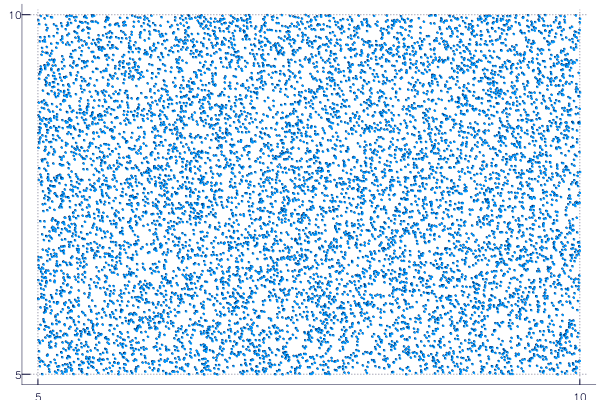
\includegraphics[width=0.46\textwidth]{images/s_orig}}
	\hfill
	\subfloat[Mixed sources]{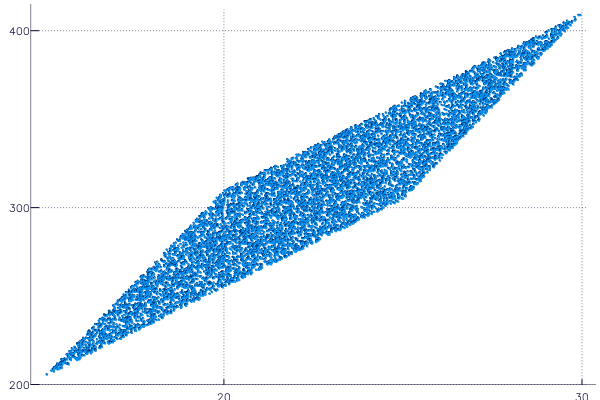
\includegraphics[width=0.46\textwidth]{images/x}} \\
	\vfill
	\subfloat[Whitening]{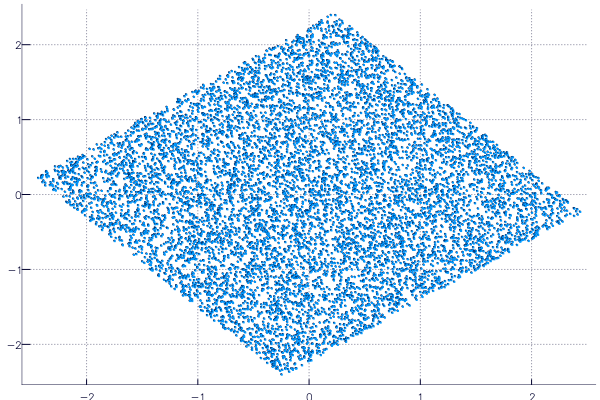
\includegraphics[width=0.46\textwidth]{images/x_w}}
	\hfill
	\subfloat[ICA]{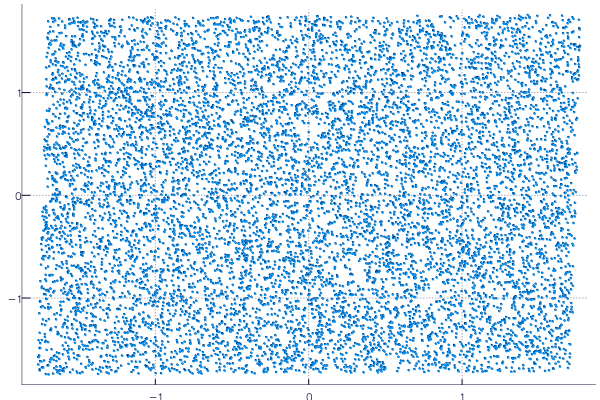
\includegraphics[width=0.46\textwidth]{images/s_retrieved}}
\end{figure}

\section{Unmixing Images}

Here we just illustrate source separation by applying it to images. We are interested in unmixing images that have been mixed linearly.

\begin{figure}[H]
	\centering
	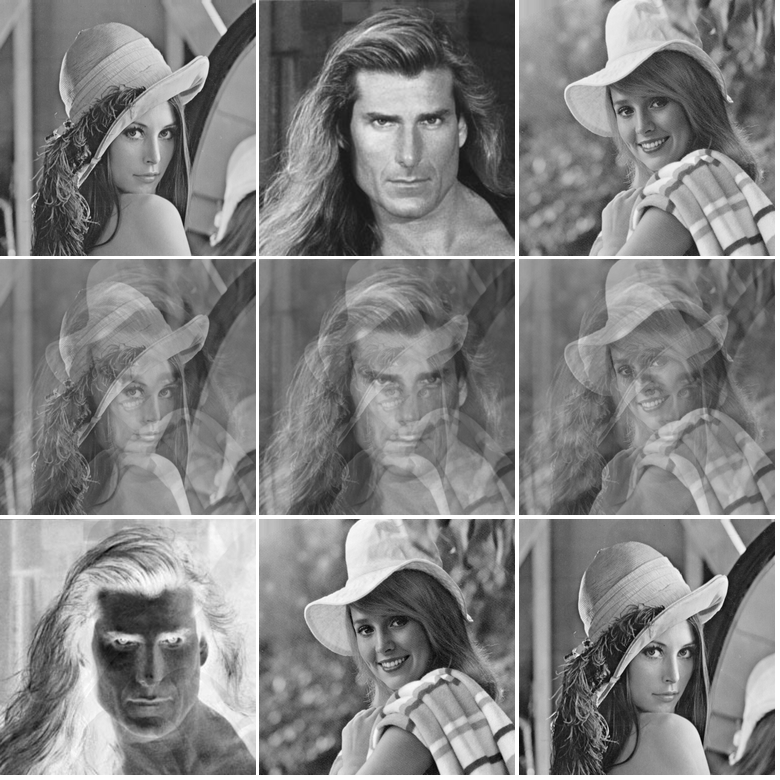
\includegraphics[width=\textwidth]{images/imagemixing}
	\caption{Original images, mixed then unmixed.}
\end{figure}

\section{Finding a natural basis of images}

In this problem the quantity of interest isn't $s$ anymore but $A$ or $w$. We interpret this problem as finding a basis of images (if we use $A$) or of detectors (if we use $w$) and $s$ being the realizations of the coefficients for this basis. We actually either find a basis of edges or the corresponding Gabor filters, \cite{Bell}.

\begin{figure}[H]
	\centering
	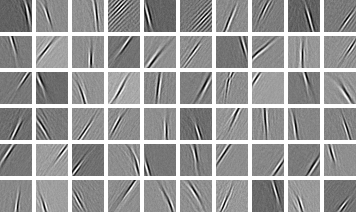
\includegraphics[width=\textwidth]{images/basis}
	\caption{Gabor filters for the previous images.}
\end{figure}

\section{Comparing Kernel-ICA and Fast-ICA}

In the accompanying \texttt{Jupyter Notebook} I give an example of comparison of Fast-ICA and Kernel-ICA. For that we need a way of measuring the performance of the algorithms. If we know the real $w$ we can use the Amari distance (which isn't a real distance) as it is invariant by scaling and permutation, the two indeterminate of our problem.

We give here the Amari distance:

\begin{align*}
	d(V,W) = \frac{1}{2 m} \sum_{i = 1}^m \left( \frac{\sum_{j = 1}^m \lvert a_{ij} \rvert}{\max_j \lvert a_{ij} \rvert} - 1 \right) + \frac{1}{2 m} \sum_{j = 1}^m \left( \frac{\sum_{i = 1}^m \lvert a_{ij} \rvert}{\max_i \lvert a_{ij} \rvert} - 1 \right)
\end{align*}

We compare both algorithms on a hard distribution (with zero excess kurtosis).

\begin{figure}[H]
	\centering
	\subfloat[Original sources]{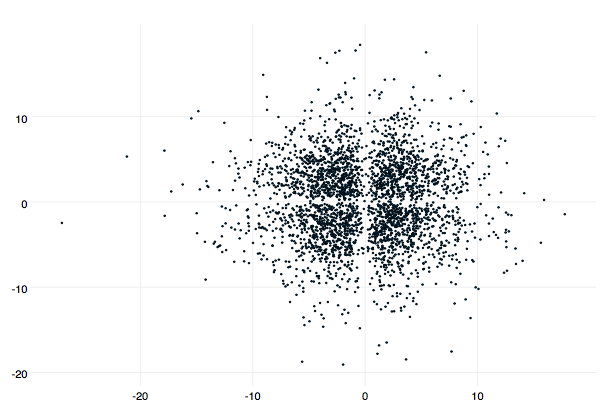
\includegraphics[width=0.46\textwidth]{images/sg_orig}}
	\hfill
	\subfloat[Mixed sources]{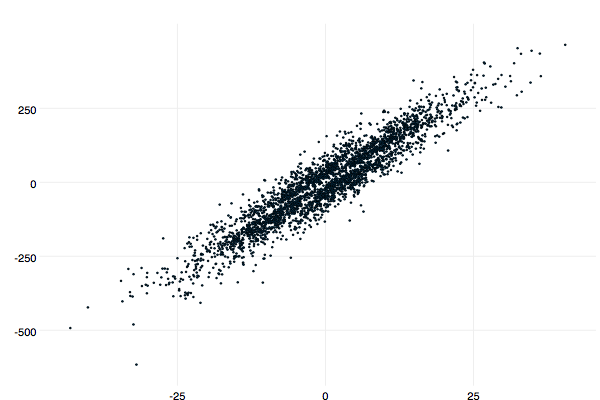
\includegraphics[width=0.46\textwidth]{images/sg_mixed}} \\
	\vfill
	\subfloat[Fast-ICA]{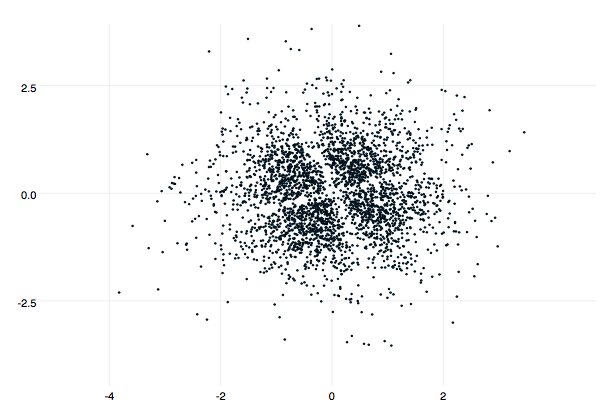
\includegraphics[width=0.46\textwidth]{images/sg_fica}}
	\hfill
	\subfloat[Kernel-ICA]{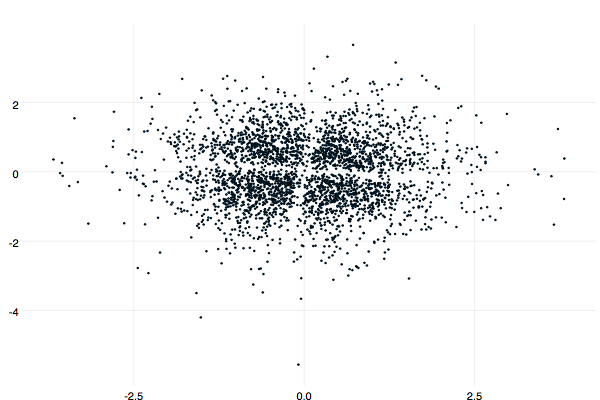
\includegraphics[width=0.46\textwidth]{images/sg_kica}}
\end{figure}

\section{Cocktail party and more}

I have other examples less suitable for a paper report in the accompanying notebook.

\listoftodos

\printbibliography

\end{document}